\section{\SysName}

\begin{figure}[tb]
    \centering
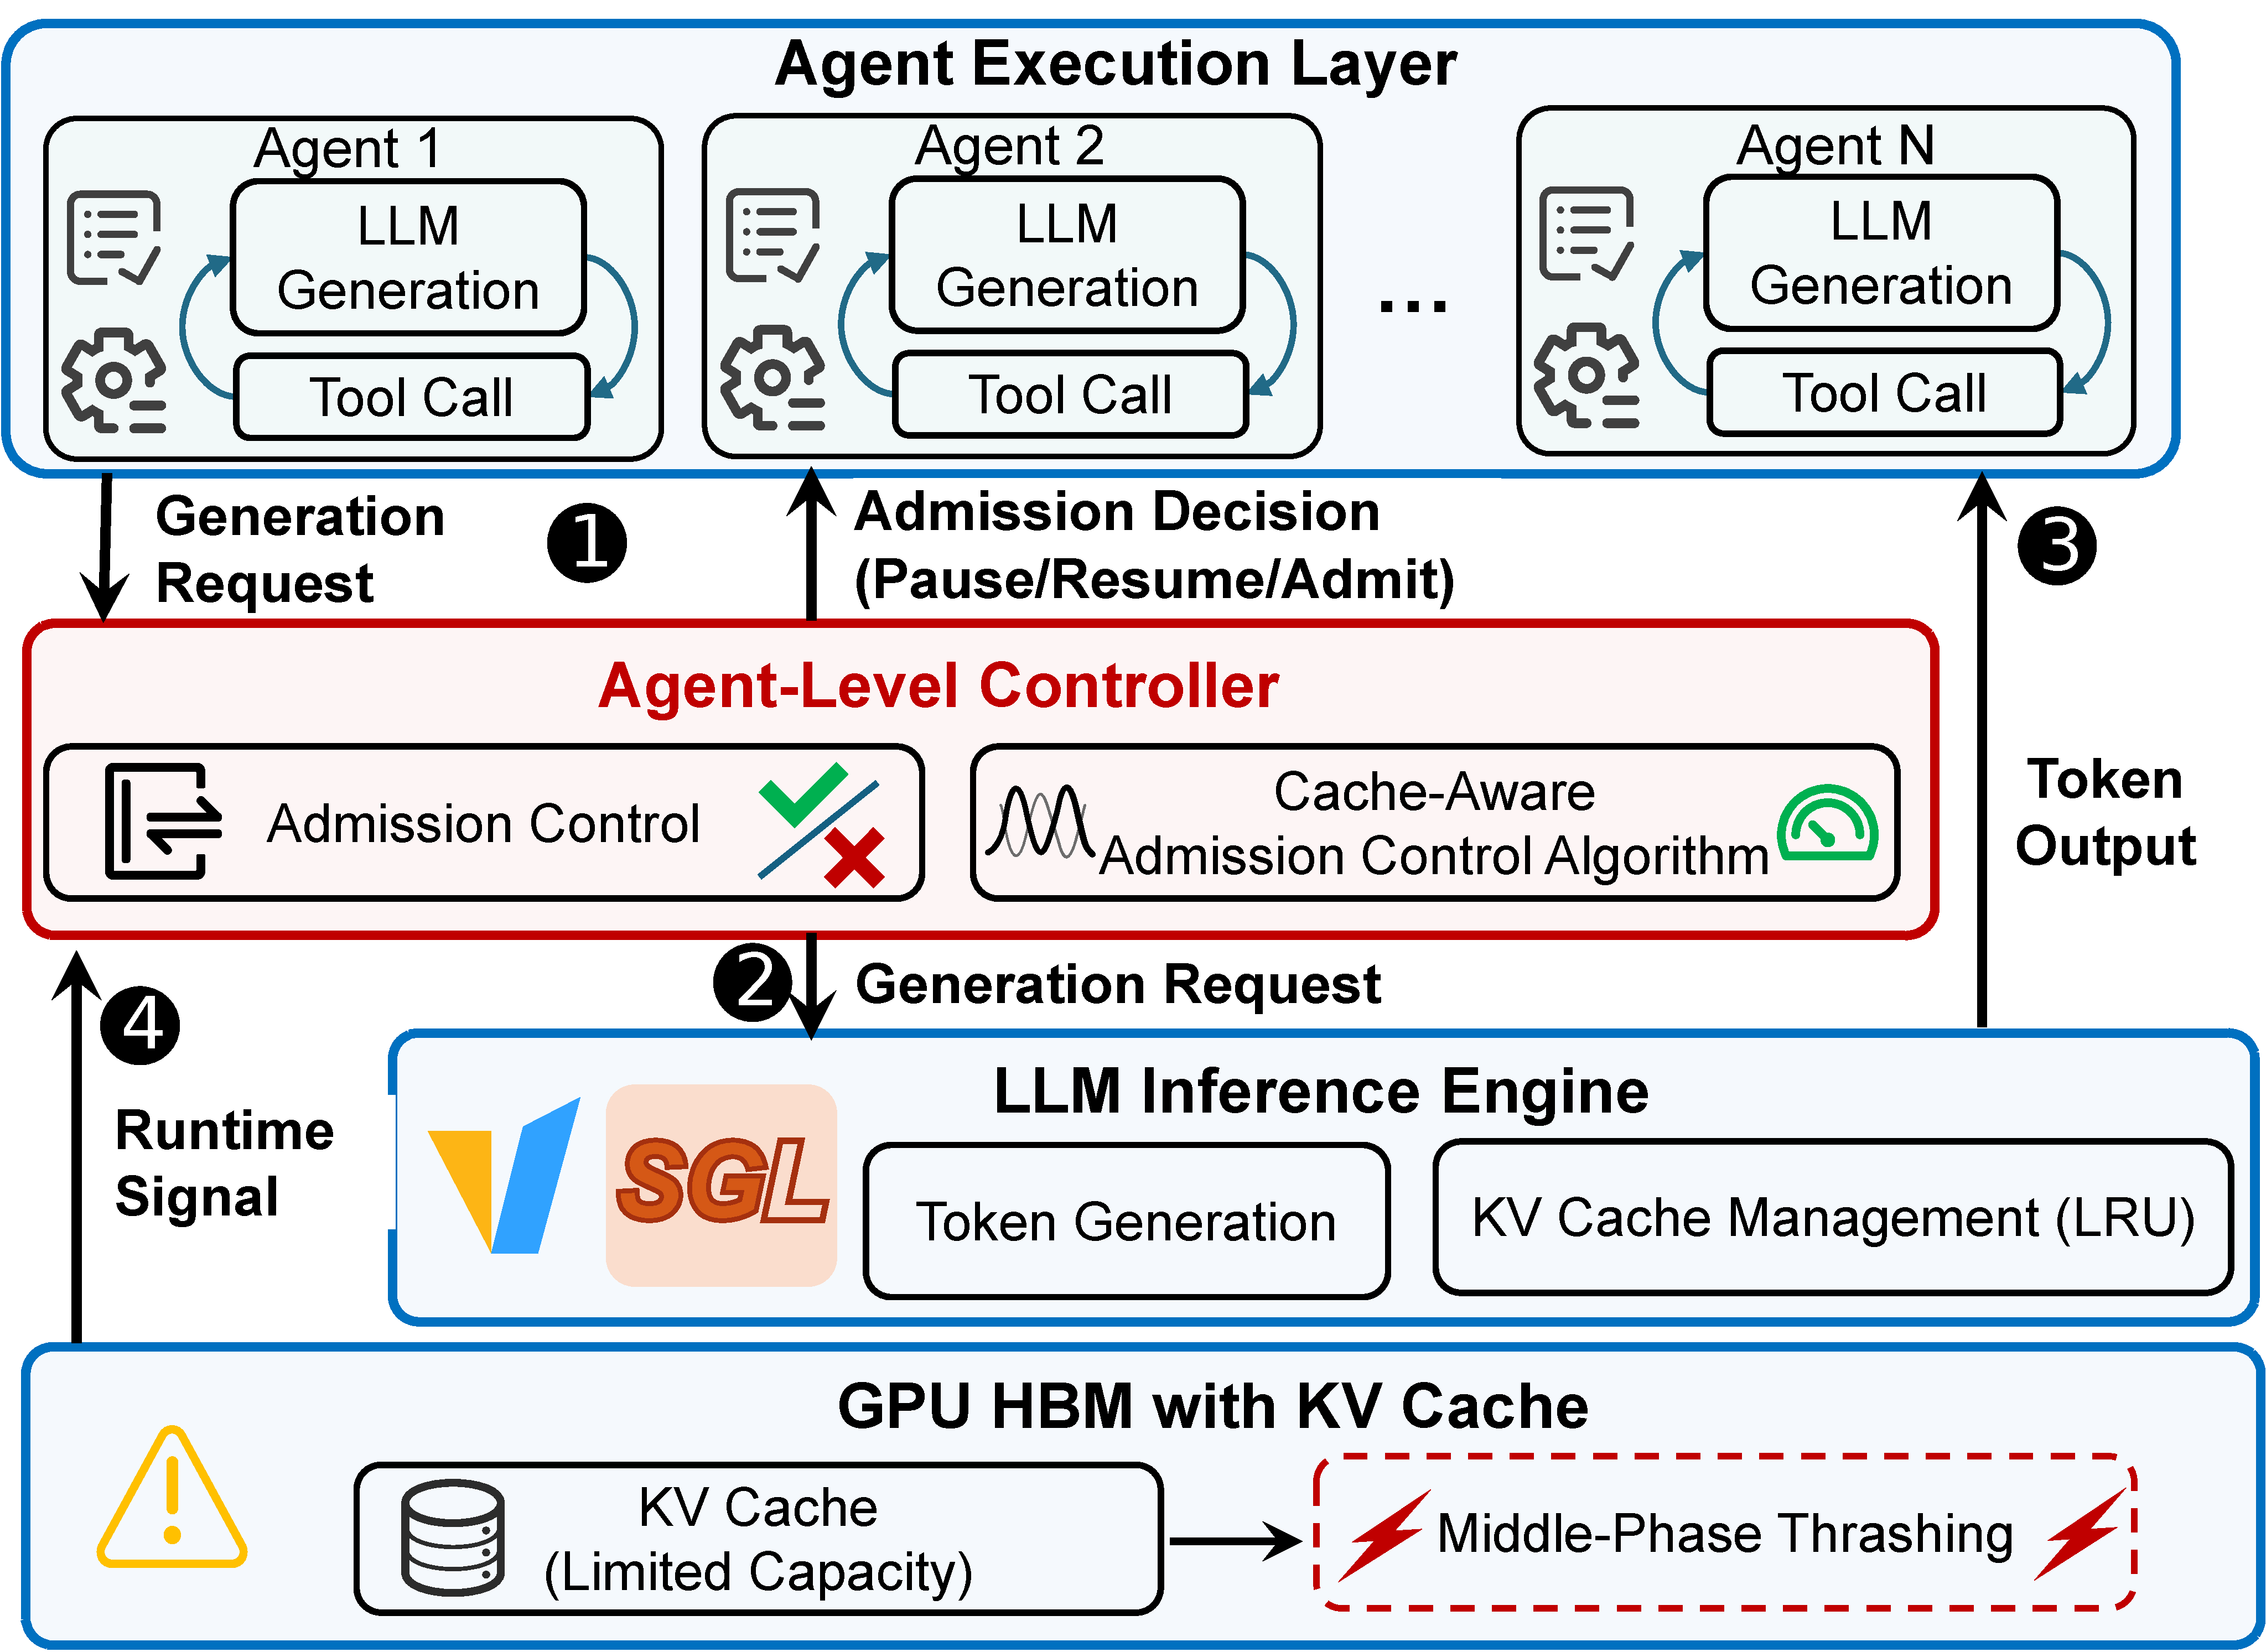
\includegraphics[width=0.98\linewidth]{figure/SystemOverview.pdf}
    \caption{System Overview.}
    \label{fig:systemoverview}
    % \vvspace{}
\end{figure}

\subsection{System Overview}
Figure \ref{fig:systemoverview} illustrates the system context in which \SysName{} operates.
Rather than introducing a new end-to-end serving stack, our design \emph{interposes a lightweight Agent-Level Controller} between existing agent execution frameworks and LLM serving engines.
The overall system can be conceptually decomposed into three components: an agent execution layer, an agent-level controller, and an LLM serving engine.


(1) \textbf{Agent Execution Layer.}
At the top of the system, multiple agents execute long-horizon workflows following the ReAct-style loop.

(2) \textbf{LLM Serving Engine.}
The LLM serving engine (e.g., SGLang) is responsible for token generation and manages the KV cache in GPU memory.

(3) \textbf{Agent-Level Controller.}
 To mitigate middle-phase thrashing, this controller manages admission at the \emph{agent granularity}. Unlike request-level schedulers, it preserves agent continuity across generation steps. By continuously monitoring real-time KV cache usage and hit rates, the controller dynamically regulates the aggregate active agent concurrency to prevent \emph{middle-phase thrashing}.
% (3) \textbf{Agent-Level Controller.}
% To mitigate middle-phase thrashing in Section~\ref{sec:motivation}, we introduce an explicit lightweight Agent-Level Controller between the agent execution layer and the serving engine. Unlike traditional request-level controllers, the controller treats the \emph{agent} as the fundamental unit of admission and control, preserving agent continuity across multiple generation steps. The controller continuously monitors runtime signals exposed by the serving engine, including KV cache usage and cache hit rate. Based on these feedback signals, it dynamically regulates the number of agents allowed to execute generation steps at any given time actively.

\noindent\textbf{Execution Workflow.} The system operates in a four-stage loop. 
\circled{1} \textbf{Agent Admission.} 
Agents submit generation requests to the controller instead of the serving engine. Based on the system state, the controller either admits the agent for execution or pauses it, preserving its execution state.
\circled{2} \textbf{Batched Generation.} 
Admitted agents proceed to batched token generation in the serving engine, consuming GPU-resident KV cache proportional to their context length.
\circled{3} \textbf{Tool Execution and Suspension.} 
Agents invoking external tools become temporarily inactive but retain their logical KV cache associations. The controller protects these idle states from eviction by restricting new admissions during high-pressure regimes.
\circled{4} \textbf{Feedback and Control Update.} 
The controller monitors runtime signals, specifically KV cache usage and hit rate. It then updates the admission policy via the adaptive mechanism (Section~\ref{subsec:AIMD}) to prevent thrashing while sustaining high throughput.
% \noindent\textbf{Execution Workflow.} The system operates in a looped workflow consisting of four stages. \circled{1} Agent Admission.
% When an agent is ready to perform a generation step, it submits the corresponding LLM request to the controller rather than directly to the serving engine.
% The controller decides whether to admit the agent based on the current system state.
% Admitted agents proceed to the serving engine, while non-admitted agents are temporarily paused at agent granularity, without discarding their execution state. \circled{2} Batched Generation.
% Admitted agents execute their generation steps in the serving engine, where token generation is batched across agents to maximize GPU utilization.
% During this phase, each agent consumes GPU-resident KV cache proportional to its current context length. \circled{3} Tool Execution and Suspension.
% After generation, agents may invoke external tools.
% During tool execution, the agent becomes inactive from the perspective of the serving engine, but its KV cache state remains logically associated with the agent.
% Without control, such inactive agents are vulnerable to cache eviction under memory pressure; the controller mitigates this risk by preventing over-admission during high-pressure regimes. \circled{4} Feedback and Control Update.
% The controller collects runtime feedback from the serving engine, including KV cache
% usage and cache hit rate. Based on these signals, the controller updates its admission policy using an adaptive control mechanism (described in Section~\ref{subsec:AIMD}), modulating concurrency to prevent KV cache thrashing while maintaining high throughput.

% The key design principle of our system is to shift from reactive cache eviction to proactive concurrency regulation.
% Rather than allowing the serving engine to overcommit GPU memory and recover via eviction or recomputation, the controller enforces a soft upper bound on the number of concurrently active agents, ensuring that the aggregate KV cache footprint remains within GPU capacity.
% This design directly addresses the middle-phase thrashing phenomenon observed in agentic batch inference and enables stable, high-throughput execution under long-horizon workloads.

% The introduced agent-level controller directly addresses middle-phase thrashing observed in agentic batch inference and enables stable, high-throughput execution under long-horizon workloads. Below, we detail each technique. 

\subsection{Agent-Level Controller}
The central challenge in offline agentic batch inference is the mismatch between the long-lived, stateful execution semantics of agents and the request-centric abstractions employed by existing LLM serving engines. To address this gap, we introduce an \emph{Agent-Level Controller} that regulates access to the serving engine at the granularity of agents rather than individual generation requests. 
% An agent encapsulates a coherent execution state that persists across multiple generation requests, including its growing context and associated KV cache footprint.
% By reasoning at agent granularity, the system can preserve execution continuity and explicitly account for long-lived memory demands that are invisible at the request level. 
Agent-level control enables the system to reason about the aggregate working set of concurrently active agents instead of requests only.
Rather than reacting to memory pressure through cache eviction or recomputation, the controller can proactively regulate how many agents are allowed to execute generation steps at any point in time.
This ensures that the combined KV cache footprint remains within GPU memory capacity, directly preventing the onset of middle-phase thrashing.

\noindent\textbf{Proactive Admission Control.} The controller implements a proactive admission control mechanism.
When an agent is ready to perform a generation step, it submits the request to the controller instead of directly entering the serving engine.
The controller decides whether to admit the agent based on current system conditions.
Admitted agents proceed to the serving engine and participate in batched generation, while non-admitted agents are temporarily paused at agent granularity, without discarding their execution state.


Figure~\ref{fig:twoagent}b illustrates an example of agent-level admission control.
At the beginning, the controller admits only Agents A1 and A2, allowing their generation requests to be continuously scheduled by the inference engine while ensuring that the combined KV cache footprint stays within the system’s GPU memory budget.
Additional agents (e.g., A3) remain pending and do not issue inference requests, preventing KV cache overcommit.
Once A2 completes its execution and releases its KV cache, the controller admits A3 from the pending set.
As a result, the system consistently maintains at most two active agents, ensuring stable memory usage and avoiding eviction-induced recomputation.


\subsection{Cache-Aware Admission Control Algorithm}
\label{subsec:AIMD}

A static admission limit proves fundamentally insufficient for agentic workloads due to the conflict between dynamic memory demands and strict capacity constraints.
First, the memory footprint of an agent is not fixed but grows monotonically as execution progresses; a concurrency limit that is safe during the initial phase will inevitably trigger memory saturation as context lengths increase.
Second, agents advance asynchronously, interleaving generation with external tool execution, causing the aggregate memory demand to fluctuate unpredictably even under a fixed number of agents.
Consequently, the system faces a dilemma: a conservative static limit wastes valuable GPU memory (under-utilization), while an aggressive limit risks crossing the saturation threshold.
% Crucially, crossing this threshold triggers \emph{middle-phase thrashing}, where the quadratic cost of context recomputation ($O(L^2)$) causes performance to collapse.
To navigate this narrow trade-off between maximizing utilization and preventing thrashing, the system requires a dynamic mechanism that continuously tracks the evolving effective capacity.

We formulate the scheduling of concurrent agents as a resource allocation problem under strict memory constraints. We draw a rigorous parallel between agent admission control and TCP Congestion Control in computer networks. In this analogy, the shared KV cache functions as the network bandwidth, while active agents act as independent data flows competing for this finite resource.

\noindent\textbf{Problem Formulation.}
We map the dynamics of agent execution to network flow control as follows:
\begin{itemize}[nosep]
    \item[(1)] \textbf{Congestion Window ($W_t$)} corresponds to the number of active agents allowed to execute concurrently.
    \item[(2)] \textbf{Packet Loss} corresponds to \emph{Cache Eviction}, where the serving engine is forced to discard active context due to memory saturation.
    \item[(3)] \textbf{Retransmission} corresponds to \emph{KV Cache Recomputation}.
\end{itemize}

\noindent\textbf{Algorithm Design.} Based on the traditional Additive Increase Multiplicative Decrease (AIMD) algorithm in TCP Congestion Control, we propose a \emph{Cache-Aware Admission Control} algorithm. It regulates the window size $W_t$ based on two real-time feedback signals from the serving engine: the \emph{KV Cache Usage} ($U_t$), which serves as a proactive congestion signal, and the \emph{Cache Hit Rate} ($H_t$), which serves as a reactive failure signal.
The control law is defined as a state-dependent transition function:
\begin{equation}
W_{t+1} = \begin{cases} 
    W_t + \alpha & \text{if } U_t < U_{low} \\
    W_t \times \beta & \text{if } U_t > U_{high} \land H_t < H_{thresh} \\
    W_t & \text{otherwise}
\end{cases}
\end{equation}
% Crucially, unlike network packet retransmission which incurs a linear cost, KV cache recomputation in Transformer-based models incurs a quadratic penalty ($O(L^2)$) relative to the sequence length. Therefore, the system penalty for ``congestion collapse'' (i.e., KV cache thrashing) is significantly higher in agent serving than in traditional networks, necessitating a conservative configuration of control thresholds to strictly avoid the thrashing regime.

% \noindent Accordingly, In our implementation, we set the additive factor $\alpha=2$ and the multiplicative factor $\beta=0.5$. The thresholds are configured as $U_{low}=0.2$, $U_{high}=0.6$, and $H_{thresh}=0.2$.

\noindent\textbf{Interpretation.}
Each component of this control law targets a specific dynamic of agent execution:

\begin{enumerate}[leftmargin=*, nosep]
    \item[(1)] \textbf{Linear Exploration ($\alpha$):} 
    When underutilized ($U_t < U_{low}$), the system employs an additive increase to linearly probe the unknown effective capacity. This allows the scheduler to maximize GPU memory utilization while avoiding the risk of sudden overshoots inherent to exponential growth.

    \item[(2)] \textbf{Minimizing Quadratic Penalty ($\beta$):} 
    Unlike network packet loss, cache thrashing incurs a convex penalty function due to the $O(L^2)$ cost of recomputation. Consequently, upon detecting thrashing, the controller applies a multiplicative cut. This forces the system to exit the high-cost regime exponentially fast ($O(\log N)$ steps), strictly minimizing the cumulative compute wasted on recomputation.

    \item[(3)] \textbf{Stabilization and Saturation:}
     The gap between $U_{low}$ and $U_{high}$ acts as an allocation buffer. Since admitting long-context agents causes discrete memory spikes rather than smooth increments, this buffer prevents these spikes from instantly triggering the penalty regime ($U_{t} > U_{high}$). Furthermore, this state allows the system to sustain high concurrency at saturation provided the hit rate remains healthy, prioritizing throughput over preemptive throttling.
   
\end{enumerate}


\noindent\textbf{Agent-Level Control Primitives.}
To regulate agent execution without entangling request-level scheduling, the controller exposes three minimal agent-level primitives: \emph{admit}, \emph{pause}, and \emph{resume}. These primitives operate on agent lifecycles rather than individual generation requests and suffice to control concurrency and memory pressure. \emph{Admit} authorizes an agent’s next generation step. \emph{Pause} temporarily suspends an agent from issuing further requests while preserving its execution state, and is applied only at well-defined boundaries between generation steps and tool execution to avoid interrupting in-flight computation. \emph{Resume} reactivates a paused agent once resources become available, with reactivation coordinated by admission control to prevent renewed cache congestion. Together, \emph{pause} and \emph{resume} allow the controller to dynamically adjust the active agent set under changing workload conditions.
